        \begin{frame}{introduction}{chain of musical communication}
              \vspace{-3mm}
                \begin{figure}
                        \centering
                        \begin{picture}(140,35)
                            %boxes
                            %\only<1>{\color{gtgold}
                            {\put(0,30){\ovalbox{\footnotesize{\parbox{20mm}{\vspace{2mm}\centering{\only<1>{\textcolor{gtgold}}{composition}}}}}}}
                            %}
                            \put(30,30){\ovalbox{\footnotesize{\parbox{20mm}{\vspace{2mm}\centering{\only<2>{\textcolor{gtgold}}{performance}}}}}}
                            \put(60,30){\ovalbox{\footnotesize{\parbox{20mm}{\vspace{2mm}\centering{\only<3>{\textcolor{gtgold}}{production}}}}}}
                            \put(90,30){\ovalbox{\footnotesize{\parbox{20mm}{\vspace{2mm}\centering{\only<4>{\textcolor{gtgold}}{distribution}}}}}}
                            \put(120,30){\ovalbox{\footnotesize{\parbox{20mm}{\vspace{2mm}\centering{\only<4>{\textcolor{gtgold}}{consumption}}}}}}
                
                            % horizontal
                            \put(22.4,30.6){\vector(1,0){7.8}}
                            \put(52.4,30.6){\vector(1,0){7.8}}
                            \put(82.4,30.6){\vector(1,0){7.8}}
                            \put(112.4,30.6){\vector(1,0){7.8}}
                        \end{picture}
                    \end{figure}
                    \vspace{-27mm}
            \begin{itemize}
                \item<1-> \textbf{creation of musical ideas} (``score'')
                    \begin{itemize}
                        \item   defines style and idea
                    \end{itemize}
                \smallskip
                \item<2-> \textbf{realization of musical ideas} into acoustical rendition 
                    \begin{itemize}
                        \item   interpretation, modification, addition, and dismissal of score information
                        \item   unique acoustic representation of score
                    \end{itemize}
                \smallskip
                \item<3-> \textbf{recording, mixing, and editing} (in case of record media)
                    \begin{itemize}
                        \item   editing and splicing of recorded data; timbre, equalization choices
                        \item   not separable from performance in a recording
                    \end{itemize}
                \smallskip
                \item<4-> \textbf{distribution \& listening}
                    \begin{itemize}
                        \item   music recommendation and discovery
                    \end{itemize}
            \end{itemize}
            \inserticon{directions}
        \end{frame}
        \begin{frame}{introduction}{musical communication and AI}
              \vspace{-3mm}
                \begin{figure}
                        \centering
                        \begin{picture}(140,35)
                            %boxes
                            %\only<1>{\color{gtgold}
                            {\put(0,30){\ovalbox{\footnotesize{\parbox{20mm}{\vspace{2mm}\centering{\only<1>{\textcolor{gtgold}}{composition}}}}}}}
                            %}
                            \put(30,30){\ovalbox{\footnotesize{\parbox{20mm}{\vspace{2mm}\centering{\only<2>{\textcolor{gtgold}}{performance}}}}}}
                            \put(60,30){\ovalbox{\footnotesize{\parbox{20mm}{\vspace{2mm}\centering{\only<3>{\textcolor{gtgold}}{production}}}}}}
                            \put(90,30){\ovalbox{\footnotesize{\parbox{20mm}{\vspace{2mm}\centering{\only<4>{\textcolor{gtgold}}{distribution}}}}}}
                            \put(120,30){\ovalbox{\footnotesize{\parbox{20mm}{\vspace{2mm}\centering{\only<5>{\textcolor{gtgold}}{consumption}}}}}}
                
                            % horizontal
                            \put(22.4,30.6){\vector(1,0){7.8}}
                            \put(52.4,30.6){\vector(1,0){7.8}}
                            \put(82.4,30.6){\vector(1,0){7.8}}
                            \put(112.4,30.6){\vector(1,0){7.8}}
                        \end{picture}
                    \end{figure}
                    \vspace{-27mm}
        \vspace{-5mm}
        \begin{columns}
        \column{.7\linewidth}
            %\begin{itemize}
                %\item[]   AI can advance all links of the musical communication chain:
                \begin{itemize}
                \item<1->   {\textbf{composition}}
                    \begin{itemize}
                        \item   intelligent assistance, e.g., ideas, auto-arrangements 
                        \item   automatic composition 
                    \end{itemize}
                \item<2->   {\textbf{performance}}
                    \begin{itemize}
                        \item   interactive music education systems
                        %\item   enable new ways of controlling sound
                        %\item   interact with artificial performers
                        \item   generation of 'human' performance
                    \end{itemize}
                \item<3->   \textbf{production}
                    \begin{itemize}
                        %\item   parametrize and suggest
                        \item   auto-edit and auto-mix
                    \end{itemize}
                \item<4->   \textbf{distribution}
                    \begin{itemize}
                        \item   match music style and consumer
                    \end{itemize}
                \item<5->   \textbf{consumption}
                    \begin{itemize}
                        \item   intelligent music discovery \& adaptable music
                    \end{itemize}
                    \end{itemize}
            %\end{itemize}
        \column{.3\linewidth}
            \only<1-2>{\begin{itemize}
                \only<1>{\item example:\\ DeepBach \includevideo{deepbach}}
                \only<2>{\item example:\\ Hatsune Miku \includevideo{hatsunemiku}}
            \end{itemize}}
            \only<3->{\bigskip\bigskip\bigskip}
                \begin{figure}
                    \vspace{13mm}
                    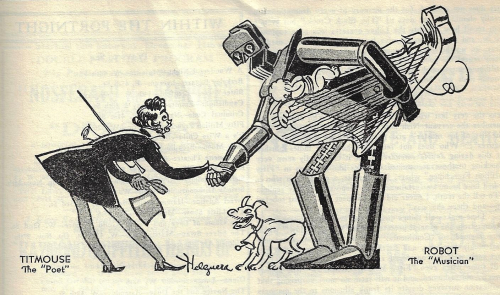
\includegraphics[scale=.7]{graph/musical-robots}
                \end{figure}
                \addreference{\href{https://longstreet.typepad.com/thesciencebookstore/2017/06/the-invasion-of-musical-robots-1929.html}{longstreet.typepad.com/thesciencebookstore/2017/06/the-invasion-of-musical-robots-1929.html}}
        \end{columns}
        \end{frame}


{ % all template changes are local to this group.
    \setbeamertemplate{navigation symbols}{}
    \begin{frame}<article:0>[plain]
        \begin{tikzpicture}[remember picture,overlay]
            \node[at=(current page.center)] {
                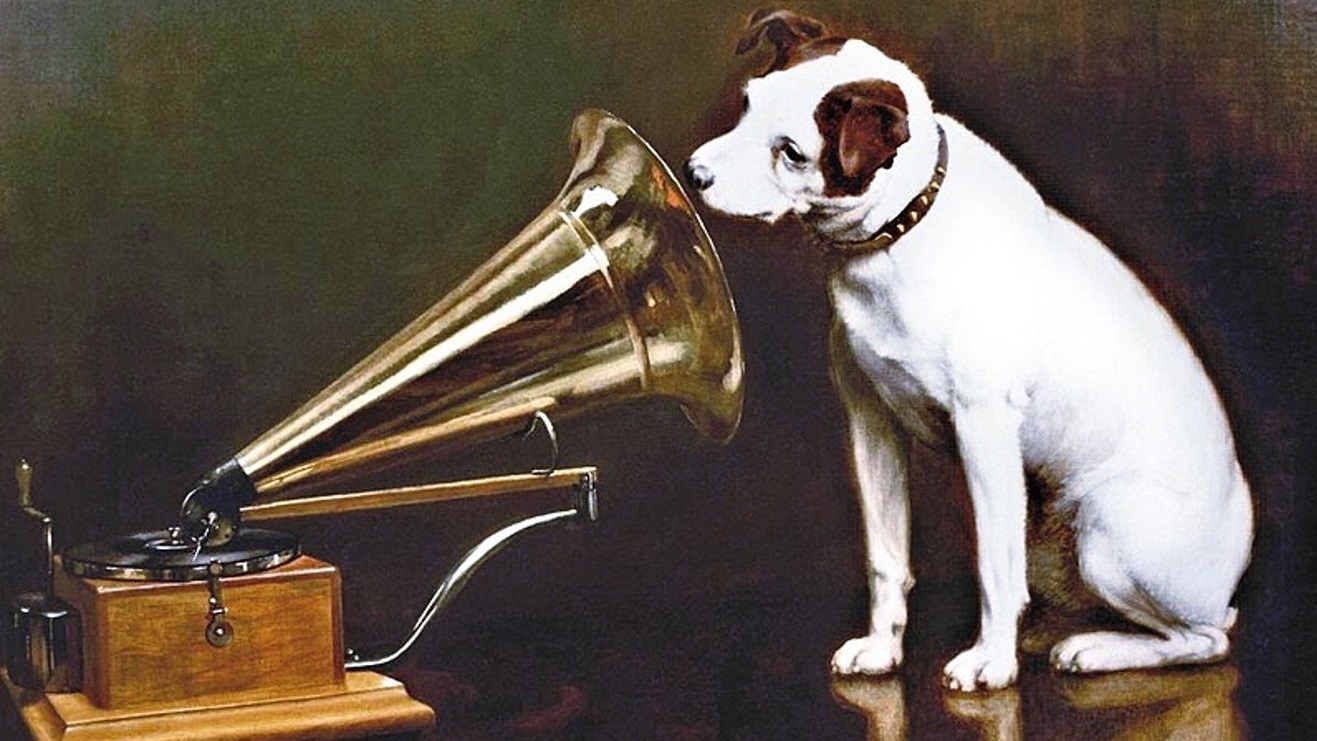
\includegraphics[keepaspectratio,
                                 width=\paperwidth,
                                 height=\paperheight]{graph/gramophone.jpg}
            };
        \end{tikzpicture}
        
        \Large{\textcolor{gtgold}{\textbf{How can we teach a computer\\ to listen to and\\ understand music?}}}
     \end{frame}
}

				%\begin{frame}{introduction}{audio classification}
            %\begin{itemize}
                %\item   audio classification: one of the earliest and seminal tasks in Music Information Retrieval (MIR)
                %\bigskip
                %\item   includes, e.g.,
                    %\begin{itemize}
                        %\item   music/speech classification
                        %\item   genre classification
                        %\item   musical instrument recognition
                        %\item   mood recognition
                        %\item   music auto-tagging
                        %\item   artist classification
                        %\item   \ldots
                    %\end{itemize}
                %\bigskip
                 %\item<2->  non-music related
                    %\begin{itemize}
                        %\item   speaker detection
                        %\item   audio event detection
                        %\item   \ldots
                    %\end{itemize}
            %\end{itemize}
        %\end{frame}

\section{audio analysis}        
        \begin{frame}{introduction}{audio classification --- traditional}
            \vspace{-3mm}\begin{textblock*}{100mm}(.5cm,2.5cm)
                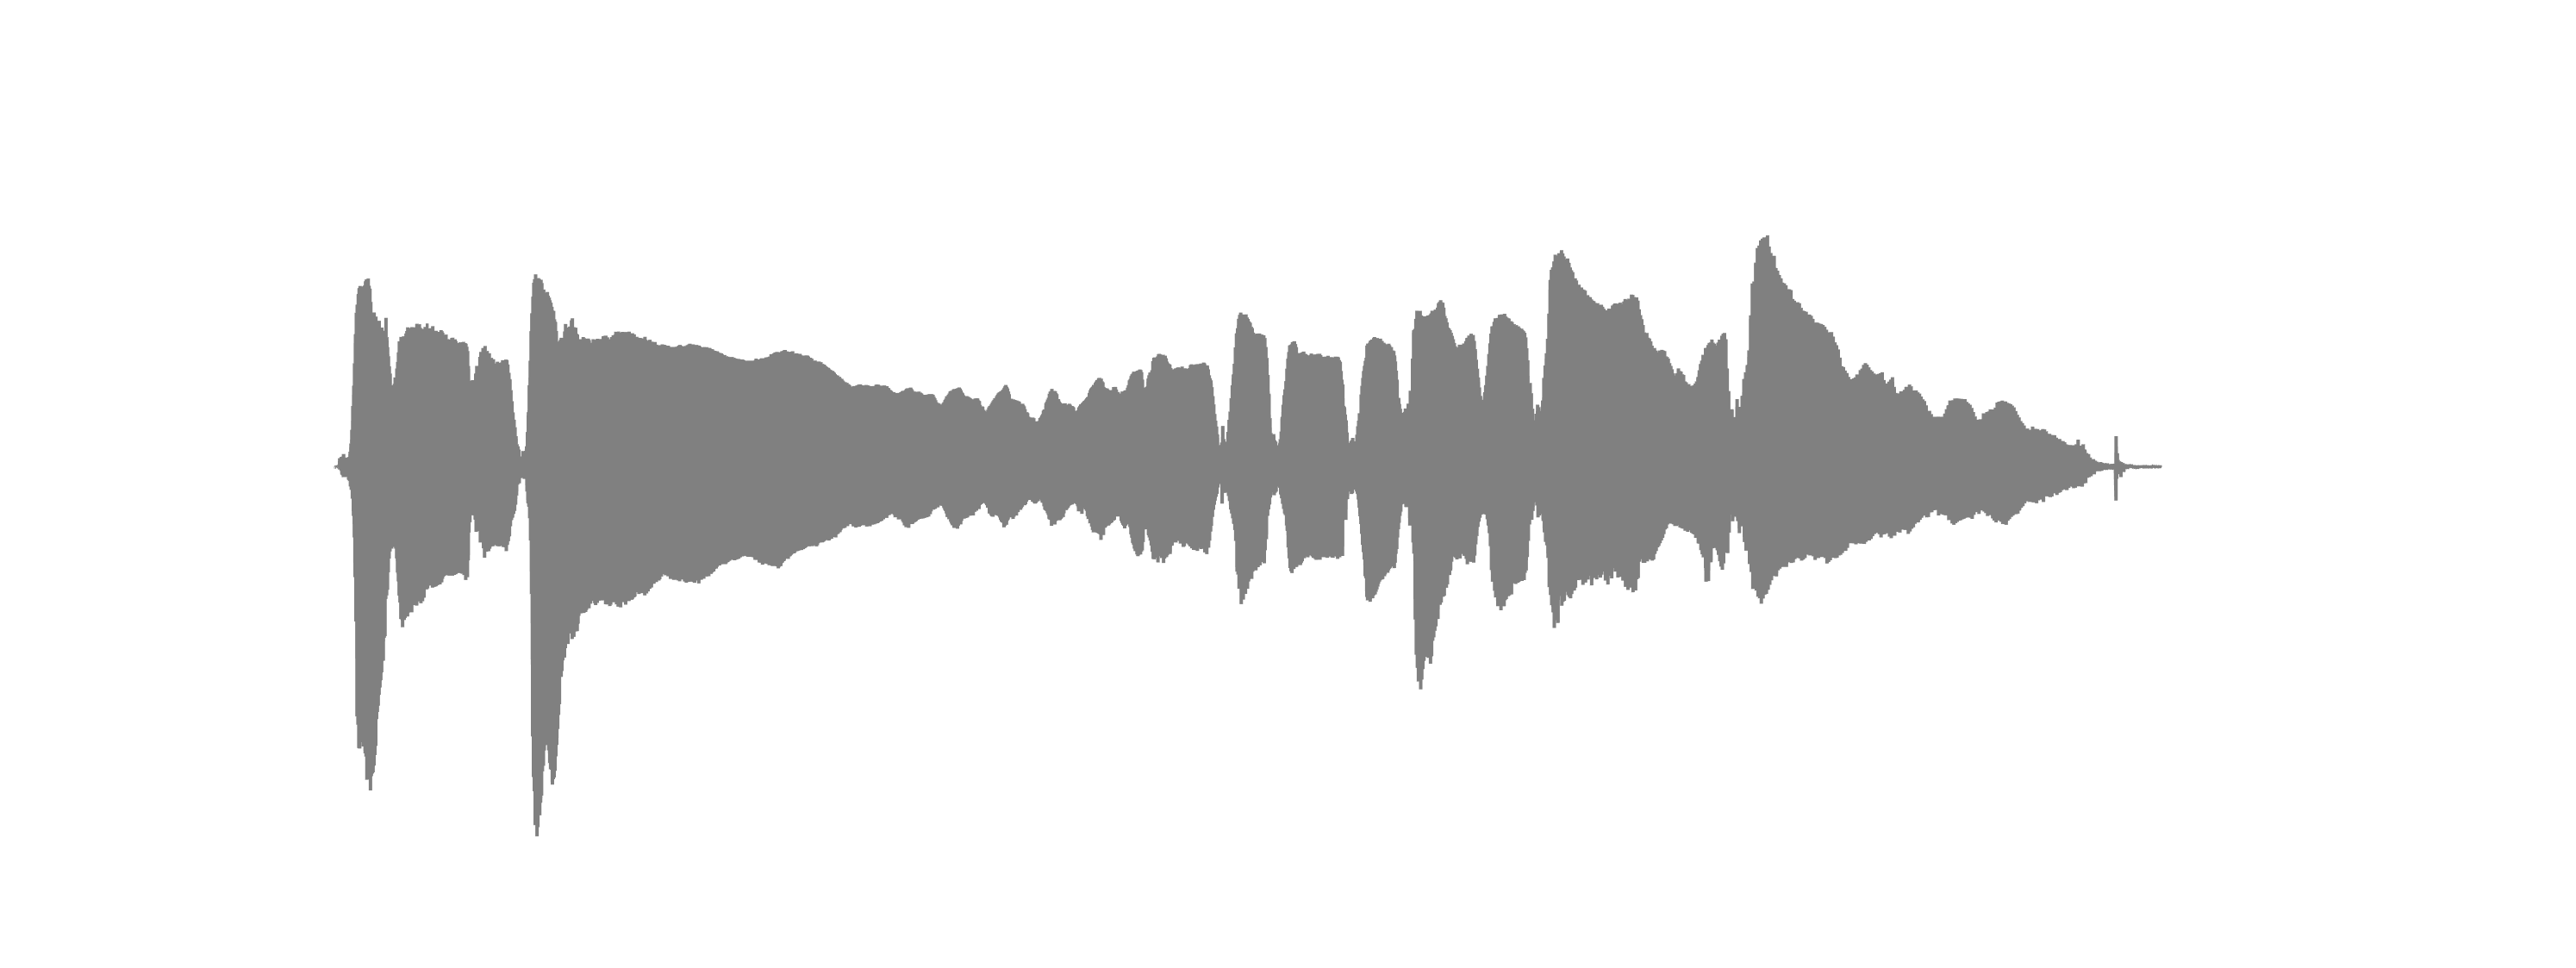
\includegraphics[scale=.2]{waveform}
            \end{textblock*}
            \begin{figure}
                \centering
								\begin{footnotesize}
									\begin{picture}(96,26)
										\setcounter{iXOffset}{0}
										\setcounter{iYOffset}{5}
										\setcounter{iXBlockSize}{28}
										\setcounter{iYBlockSize}{16}
										\setcounter{iYBlockSizeDiv2}{8}
										\setcounter{iDistance}{8}

										\addtocounter{iYOffset}{\value{iYBlockSizeDiv2}}
										\addtocounter{iYOffset}{-2}

										%\addtocounter{iXOffset}{-1}
										\put(\value{iXOffset}, \value{iYOffset})
											{\text{{\shortstack[c]{audio\\ signal}}}}
										\addtocounter{iXOffset}{1}

										\addtocounter{iYOffset}{2}
										\addtocounter{iXOffset}{\value{iDistance}}

										\put(\value{iXOffset}, \value{iYOffset})
											{\vector(1,0){\value{iDistance}}}

										\addtocounter{iXOffset}{\value{iDistance}}
										\addtocounter{iYOffset}{-\value{iYBlockSizeDiv2}}
										
										\put(\value{iXOffset}, \value{iYOffset})
											{\framebox(\value{iXBlockSize}, \value{iYBlockSize}) {\shortstack[c]{feature extraction}}}

										\addtocounter{iXOffset}{\value{iXBlockSize}}
										\addtocounter{iYOffset}{\value{iYBlockSizeDiv2}}

										\put(\value{iXOffset}, \value{iYOffset})
											{\vector(1,0){\value{iDistance}}}

										\addtocounter{iXOffset}{\value{iDistance}}
										\addtocounter{iYOffset}{-\value{iYBlockSizeDiv2}}

										\put(\value{iXOffset}, \value{iYOffset})
											{\framebox(\value{iXBlockSize}, \value{iYBlockSize}) {\shortstack[c]{classification,\\ inference}}}

										\addtocounter{iXOffset}{\value{iXBlockSize}}
										\addtocounter{iYOffset}{\value{iYBlockSizeDiv2}}

										\put(\value{iXOffset}, \value{iYOffset})
											{\vector(1,0){\value{iDistance}}}

										\addtocounter{iXOffset}{\value{iDistance}}
										\addtocounter{iYOffset}{-2}

										\addtocounter{iXOffset}{1}
										\put(\value{iXOffset}, \value{iYOffset})
											{\text{{\shortstack[c]{class\\ labels}}}}
										
									\end{picture}
								\end{footnotesize}
            \end{figure}
            
            \vspace{-5mm}
            \begin{columns}
                \column{.5\textwidth}
                    \begin{itemize}
                        \item<2->[]	\textbf{feature} representation
                                \begin{itemize}
                                    \item 	compact and non-redundant
                                    \item	task-relevant
                                    \item   easy to analyze
                                    \item   e.g., MFCCs etc.
                                \end{itemize}
                    \end{itemize}
                \column{.5\textwidth}
                    \begin{itemize}
                        \item<3->[]	\textbf{classification}
                                \begin{itemize}
                                    \item	map or convert feature to comprehensible domain
                                    \item   e.g., Support Vector Machines etc.
                                \end{itemize}
                    \end{itemize}
            \end{columns}
            \phantom{\footfullcite{burred_hierarchical_2004}}
        \end{frame}
        
        \begin{frame}{introduction}{neural network based approaches}
            \vspace{-3mm}
            \begin{itemize}
                \item   no custom-designed features anymore
                \item   learn features from basic inputs (like spectrograms)
            \end{itemize}
            \begin{figure}%
                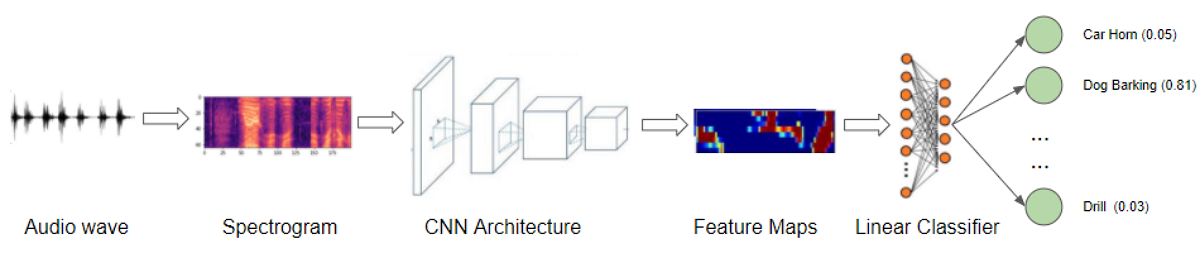
\includegraphics[width=\columnwidth]{audio_classification}%
            \end{figure}
            \addreference{Fig.: \href{https://towardsdatascience.com/audio-deep-learning-made-simple-sound-classification-step-by-step-cebc936bbe5}{towardsdatascience.com}}
            \pause
            \begin{itemize}
                \item   less required expert-knowledge, more complex systems
                \item   less expert-tweaking, more rigorous experimental requirement
                \item   much \textcolor{gtgold}{\textbf{higher data requirements}}
            \end{itemize}
            
        \end{frame}
